\documentclass[11pt,a4paper]{article}
\usepackage[top=3cm, bottom=2cm, left=3cm, right=2cm]{geometry}
\usepackage[utf8]{inputenc}
% \usepackage[T1]{fontenc}
\usepackage{amsmath, amsfonts, amssymb}
\usepackage{siunitx}
\usepackage[brazil]{babel}
\usepackage{graphicx}
\usepackage[margin=10pt,font={small, it},labelfont=bf, textfont=it]{caption}
\usepackage[dvipsnames, svgnames]{xcolor}
\DeclareCaptionFont{MediumOrchid}{\color[svgnames]{MediumOrchid}}
\usepackage[pdftex]{hyperref}
\usepackage{natbib}
\bibliographystyle{plainnat}
\bibpunct{[}{]}{,}{s}{}{}
\usepackage{color}
\usepackage{footnote}
\usepackage{setspace}
\usepackage{booktabs}
\usepackage{multirow}
\usepackage{subfigure}
\usepackage{fancyhdr}
\usepackage{leading}
\usepackage{indentfirst}
\usepackage{wrapfig}
\usepackage{mdframed}
\usepackage{etoolbox}
\usepackage[version=4]{mhchem}
\usepackage{enumitem}
\usepackage{caption}
\DeclareCaptionLabelFormat{figuras}{\textcolor{CarnationPink}{Figura \arabic{figure}}}
\captionsetup[figure]{labelformat=figuras}

\makeatletter
\renewcommand\tagform@[1]{\maketag@@@{\color{CarnationPink}(#1)}}
\makeatother

\renewcommand{\theequation}{Eq. \arabic{equation}}
\renewcommand{\thefigure}{Fig. \arabic{figure}}

\setlist[itemize]{label=\textcolor{CarnationPink}{$\mathbf{\square}$}}

\setlist[enumerate]{label=\textcolor{CarnationPink}{\arabic*.}, align=left}


\newcounter{exemplo}

\NewDocumentEnvironment{exemplo}{ O{} }{%
\allowbreak
\setlength{\parindent}{0pt}
  \begin{mdframed}[
  leftline=true,
  topline=false,
  rightline=false,
  bottomline=false,
  linewidth=2pt,
  linecolor=CarnationPink,
  frametitlerule=false,
  frametitlefont=\Large\bfseries\color{CarnationPink},
  frametitle={\color{CarnationPink}\normalfont\bfseries #1},
  ]
}{%
  \end{mdframed}
}

\setlength{\fboxsep}{10pt}
\setlength{\fboxrule}{1pt}
\usepackage{float}
\renewcommand{\thefootnote}{\alph{footnote}}
\usepackage{url}
\hypersetup{
    colorlinks=true,
    linkcolor=cyan,
    filecolor=cyan,      
    urlcolor=cyan,
    citecolor=cyan,
    pdftitle={Resumos}
}
\pagestyle{fancy}
\fancyhf{}
\renewcommand{\headrulewidth}{0pt}
\rfoot{Página \thepage}

\title{Braquiterapia}
\author{Definições E Física da Braquiterapia\nocite{*}}
\date{\textit{Dalila Mendonça}}
\begin{document}
	\maketitle



	\section{Tipos de Braquiterapia}

	Os procedimentos de Braquiterapia podem ser classificados de acordo com a técnica do implante, duração do tratamento, taxa de dose e o tipo de carregamento.

		\subsection{Técnicas implantárias}

			Quanto a técnica de implante, a braquiterapia pode ser classificada como:

		\begin{enumerate}
			\item \textbf{Braquiterapia Intersticial:} Técnica cujas fontes de braquiterapia são colocadas diretamente em contato com o tecido. Exemplos:Braquiterapia de próstata, braquiterapia de cabeça e pescoço, braquiterapia de sarcomas, etc...
			
			\item \textbf{Braquiterapia Intracavitária:}  Procedimento onde as fontes são colocadas dentro de aplicadores e que são inseridos dentro de cavidades, e o aplicador em si que fica em contato com o tecido que será tratado. Exemplos: Braquiterapia ginecológica (vagina e útero), etc...
			
			
			\item \textbf{Braquiterapia Intraluminal:} Técnica que consiste na inserção das fontes com auxilio de catéteres em órgãos tubulares (lume, \textit{Do inglês - lumen}). Exemplos: Esôfago e Traqueia.
			
			\item \textbf{Braquiterapia Superficial:} Consiste na inserção das fontes de radiação em placas, moldes ou aplicadores que estarão em contato com superfícies externas para tratamento. Exemplos: Braquiterapia de pele e braquiterapia oftalmológica.
			
			\item \textbf{Braquiterapia Intravascular:} Se trata da inserção das fontes de radiação em vasos sanguíneos.

		\end{enumerate}


		\subsection{Duração do Tratamento}

			Quanto à duração do tratamento, a braquiterapia pode ser classificadas como:

			\begin{enumerate}

				\item \textbf{Braquiterapia Permanente:}  São os tratamentos no qual as fontes são permanentemente colocadas no paciente, ou seja, uma vez inseridas essas fontes não são removidas. Este procedimento envolve fontes de radiação cujo tempo de meia-vida é muito menor que o tempo de duração do implante (que se dará ao longo de todo o tempo de vida do paciente).
				
				\item \textbf{Braquiterapia Temporária:} São os tratamentos onde a fonte de radiação é implantada no paciente por um curto período de tempo e então a fonte é removida. Este procedimento envolve fontes de radiação cujo tempo de meia-vida é muito maior que a duração do implante.
				
			\end{enumerate}

		\subsection{Taxa de Dose}

			Pode ser classificada como Braquiterapia de Baixa Taxa de Dose (LDR), Braquiterapia de média taxa de Dose (MDR), Braquiterapia de Alta taxa de Dose (HDR) e Braquiterapia com Taxa de Dose Pulsada (PDR), onde:

			\begin{itemize}
				\item \textbf{LDR:} Entrega a dose com uma taxa de dose entre 0.4 Gy/h até 2 Gy/h. Devido ao longo tempo de tratamento, é necessário a internação do paciente para realizar o tratamento, embora possa ser possível um atendimento ambulatorial.
				\item \textbf{MDR:} Entrega a dose com taxas de dose que variam de 2 Gy/h até 12 Gy/h.
				\item  \textbf{HDR:} A dose é entregue com taxas de dose superiores a 12 Gy/h. Devido à tecnologia utilizada para entrega da dose é possível entregar taxas de dose superiores à 7 Gy/min diminuindo significativamente o tempo de tratamento e portanto não requer internação. 
				\item \textbf{PDR:} Esta técnica consiste em utilizar uma fonte de HDR para simular um tratamento LDR através da emissão de um pulso de radiação a cada 1 hora.
			\end{itemize}

		\subsection{Carregamento da Fonte}

			Para o carregamento da fonte no paciente são utilizados \textbf{aplicadores}, e a utilização de aplicadores se deve a dois principais motivos:

			\begin{enumerate}
				\item Os aplicadores permitem que o médico insira a fonte de radiação sem a necessidade do médico entrar em contato direto com a fonte. \textit{\textcolor{CarnationPink}{Exemplo:}} \textit{Aplicador MICK para braquiterapia de próstata,  \ref{img:aplicadorMick}.}

				\begin{figure}[h]
					\centering
					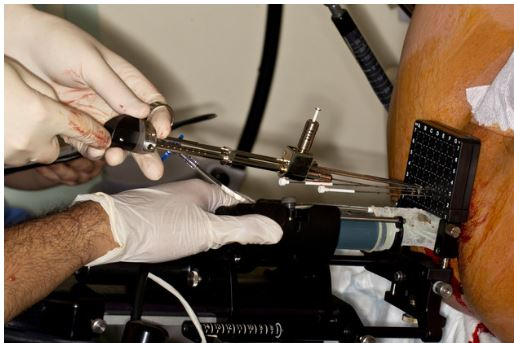
\includegraphics[width=0.5\textwidth]{Imagens/aplicadorMick.JPG}
					\caption{Aplicador MICK utilizado na Braquiterapia de próstata. São utilizadas agulhas para inserção das fontes.}
					\label{img:aplicadorMick}
				\end{figure}

				\item Os aplicadores permitem que a fonte permaneça em uma posição fixa durante todo o tratamento. \textit{\textcolor{CarnationPink}{Exemplo:}} \textit{Sonda e ovóides,    \ref{img:aplicadorSondaEOvoides}.}
				
				\begin{figure}[h]
					\centering
					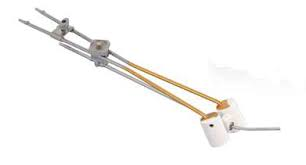
\includegraphics[width=0.5\textwidth]{Imagens/aplicadorSondaEOvoides.jpg}
					\caption{Aplicador ginecológico com sonda e ovóides.}
					\label{img:aplicadorSondaEOvoides}
				\end{figure}
			\end{enumerate}

			Os tipos de carregamento podem ser definidos com base na forma como as fontes serão inseridas e de acordo com o tempo com o qual a fonte ficará em cada posição de parada (posições pré-definidas que a fonte irá parar para entregar a dose).

			Quanto ao método de inserção das fontes, o carregamento da fonte pode ser classificado como:

			\begin{itemize}
				\item \textbf{Braquiterapia com pré-carregamento manual (\textit{preloaded}):} Onde as fontes são manualmente pré-carregadas no aplicador e na sequência o aplicador é inserido no paciente.
				\item \textbf{Braquiterapia com pós-carregamento manual (\textit{Manually afterloaded}):} Os aplicadores são inseridos no paciente e na sequência o médico insere manualmente as fontes nos aplicadores.
				\item \textbf{Braquiterapia com pós-carregamento remoto (\textit{Remotely afterloaded}):} O aplicador é inserido no paciente e um equipamento (o robô) é responsável por mover as fontes dentro do aplicador de acordo com as posições remotamente pré-definidas. Neste procedimento é envolvida uma maior tecnologia que permite uma maior precisão no posicionamento das fontes.
			\end{itemize}

			Já com base distribuição dos tempos de parada das fontes, o carregamento pode ser definido como:

		% Completar aqui o motivo dos carregamentos serem diferentes e a mudança na distribuição de dose
			\begin{itemize}
				\item \textbf{Carregamento Uniforme: } Onde as fontes com a mesma atividade permanecerão o mesmo período de tempo em cada posição de parada, gerando uma distribuição de dose mais quente no centro do aplicador e mais fria das extremidades do aplicador, como mostra a    \ref{img:carregamentoUniforme}.
				
					\begin{figure}[h]
						\centering
						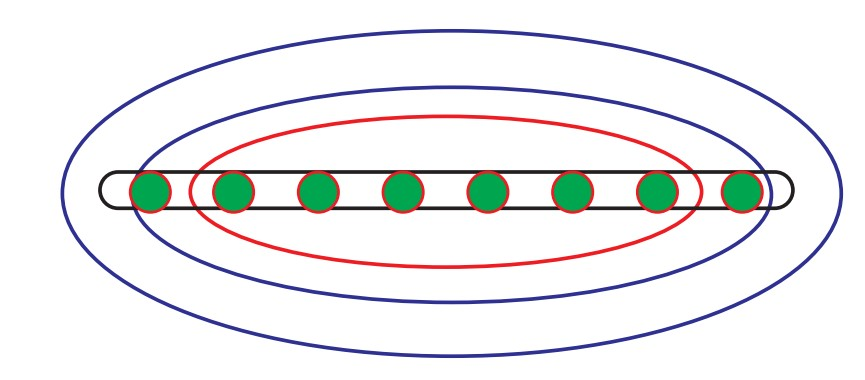
\includegraphics[width=0.4\textwidth]{Imagens/carregamentoUniforme.jpg}
						\caption{Carregamento Uniforme.}
						\label{img:carregamentoUniforme}
					\end{figure}

				\item \textbf{Carregamento Não-Uniforme:} As fontes com mesma atividade permanecem tempos diferentes em cada posição de parada. Esta técnica pode ser utilizada para gerar uma distribuição de dose mais homogênea ao longo do aplicador ao utilizar um carregamento com tempos de parada maiores nas extremidades que no centro do aplicador (carregamento periférico), como mostra a    \ref{img:carregamentoPeriferico}.
				
				\begin{figure}[h]
					\centering
					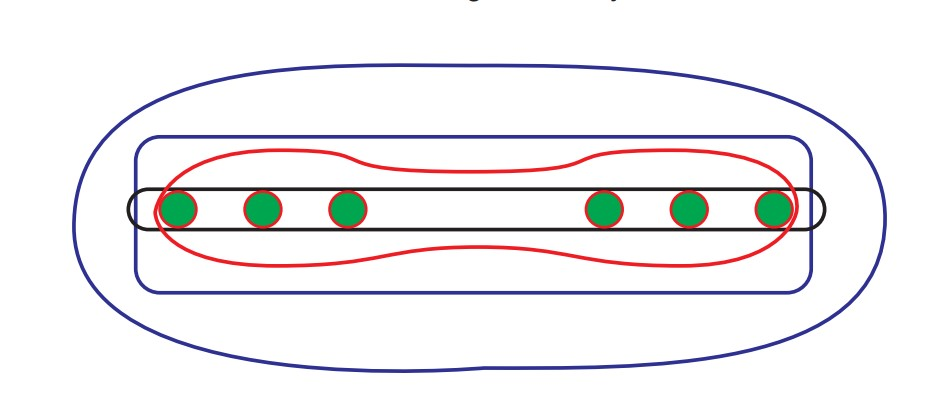
\includegraphics[width=0.4\textwidth]{Imagens/carregamentoPeriferico.jpg}
					\caption{Carregamento Periférico.}
					\label{img:carregamentoPeriferico}
				\end{figure}

			\end{itemize}
		
	\section{Radioatividade}

		A Radioatividade é o fenômeno físico por trás das emissão de radiação pelas fontes utilizadas em braquiterapia. As principais relações físicas que caracterizam o fenômeno da Radioatividade são:

		\begin{itemize}
			\item \textbf{Desintegração por unidade de tempo:} Mostra o número de átomos que se desintegram com o passar do tempo. 

				\begin{equation}
					\frac{dN}{dt} = -\lambda N
					\label{eq:DesintegraçãoPorUnidadeDeTempo}
				\end{equation}
		
				\begin{exemplo}[onde:]
					\textcolor{CarnationPink}{$\mathbf{\frac{dN}{dt}}$} é o número de desintegrações por unidade de tempo;

					\

					\textcolor{CarnationPink}{$\mathbf{\lambda}$} é a constante de decaimento; Refere-se à taxa pela qual o número de átomos radioativos diminuem ou decaem ao longo do tempo; e

					\


					\textcolor{CarnationPink}{$\mathbf{N}$} é o número de átomos radioativos da amostra.

					\

					\textit{\textbf{\textcolor{CarnationPink}{Obs:}}} O sinal negativo na   indica que o número de átomos radioativos remanescentes na amostra diminui com o passar do tempo. 
				\end{exemplo}
				

			\item \textbf{Lei do decaimento exponencial: } Permite obter o número de átomos radioativos em  um tempo t qualquer que ainda não decaíram, ou seja, indica o número de átomos de um determinado elemento instável que não sofreram transformação.

				\begin{equation}
					N(t) = N_0 \times e^{-\lambda t}
					\label{eq:decaimentoExponencial}
				\end{equation}
				
				onde,

				$N_0$ é o número inicial de átomos radioativos (t = 0);
				
				$t$ é o tempo decorrido; e

				$N(t)$ é a quantidade de átomos radioativos remanescentes após um tempo t.

				Através da   \ref{eq:decaimentoExponencial} podemos extrair que a fração de átomos que permanecem na amostra após um tempo t é dada por:

				\begin{equation}
					\frac{N(t)}{N_0}
				\end{equation}

				E a fração de átomos que decaíram da amostra é dada por:

				\begin{equation}
					1 - \frac{N(t)}{N_0}
				\end{equation}

			\item \textbf{Tempo de meia-vida ($t_{1/2}$): } É o tempo no qual o número de átomos radioativos de uma amostra demora para decair pela metade do seu valor inicial, ou seja é o tempo para que o número de átomos radioativos remanescentes na amostra fique igual a metade do seu valor inicial, 
			
				\begin{equation}
					N(t) = \frac{1}{2}N_0
				\end{equation}

				Portanto o tempo de meia-vida  ($t_{1/2}$) é dado por:

				\begin{equation}
					t_{1/2} = \frac{\ln 2}{\lambda}
				\end{equation}

				\textbf{\textcolor{CarnationPink}{Obs:} } Podemos notar que um material radioativo com uma vida longa está relacionado com um grande tempo de veia vida e portanto um pequeno valor para a taxa de decaimento.

				Após $n$ $t_{1/2}$ temos que:

				\begin{equation}
					N = \left({1/2}\right)^n N_0
				\end{equation}

% Deduzir o porque a vida média assume que N é igual a 1/e				
			\item \textbf{Tempo de vida-média ($\tau$): } Se caracteriza como o tempo necessário para que todos os átomos radioativos decaiam assumindo que a taxa de decaimento se mantenha fixa em seu valor inicial.
			
				\begin{equation}
					\tau = \frac{1}{\lambda}
				\end{equation}

				\begin{equation}
					\tau = 1.44 \times t_{1/2}
				\end{equation}

				\textbf{\textcolor{CarnationPink}{Obs:}} O tempo de vida média é utilizado para calcular a dose total recebida em um implante permanente pois as fontes radioativas ficarão em todo o seu tempo de vida inseridas no paciente e a vida média descreve o tempo médio total que um material permanece radioativo.

			\item \textbf{Meia Vida Biológica ($t_{biol}$):} É o tempo que leva para a metade da fonte ser eliminada pelo próprio corpo.
			
			\item \textbf{Meia Vida Efetiva ($t_{eff}$): } É o tempo de meia vida que considera tanto a eliminação biológica do material quanto o seu tempo de decaimento.
			
				\begin{equation}
					\frac{1}{t_{eff}} = \frac{1}{t_{1/2}} + \frac{1}{t_{biol}}
				\end{equation}

			\item \textbf{Atividade ($A$): } É definida como o número de desintegrações por unidade de tempo, ou seja, é a taxa de decaimento de uma fonte radioativa. 
				
				\begin{equation}
					A = -\frac{dN}{dt} = \lambda N
				\end{equation}

			\item \textbf{Atividade em função do tempo ($A(t)$): } Uma vez conhecida a atividade $A_0$ em um tempo $t_0$ qualquer, pode-se obter a atividade da fonte em função do tempo, seja ele no passado ou futuro, através da  :
				
				\begin{equation}
					A(t) = A_0 \times e^{-\lambda t}
					\label{eq:AtividadeNoTempo}
				\end{equation}

			\item \textbf{Atividade Específica: } É definida como a atividade de um material por unidade de massa. É uma grandeza importante para a produção de fontes de braquiterapia HDR,pois uma alta atividade específica fornece uma maior atividade em uma menor quantidade de material radioativo, permitindo uma alta taxa de dose em uma fonte pequena o suficiente para ser inserida dentro das cavidades onde ocorrerão os tratamentos.

		\end{itemize}

	\section{Especificação da Fonte}
		
		Uma fonte pode ser especificada com base na determinação da força da fonte \textit{(Source Strength)}. Essa grandeza sofreu variações ao longo do tempo, de acordo com o surgimento de novas fontes de radiação que substituíram o Rádio-226. 

		\subsection{Massa de Radio-226}

			Forma antiga de especificação da fonte que se baseia na quantidade de material presente na amostra. Era expressa em $mg\; Ra$ que quantificava a quantidade de radiação emitida quando a única fonte de radiação utilizada em braquiterapia era o $\mathrm{{}^{226}Ra}$

		\subsection{Massa de Rádio Equivalente}

			Foi introduzida quando surgiram diferentes materiais radioativos para serem utilizados em braquiterapia, como o Césio-137 (${}^{137}Cs$). Esta quantidade é definida como a massa de Rádio, encapsulada em 0.5 mm de Platina (Pt) que produz a mesma taxa de exposição produzida pela fonte de interesse na posição de calibração.

		\subsection{Atividade}

			É uma das grandezas que pode ser utilizada para especificar a fonte. Como descrito anteriormente, a Atividade é definida como o número de núcleos se submetendo ao decaimento radioativo por unidade de tempo,   \ref{eq:AtividadeNoTempo}.

			\begin{itemize}
				\item Unidade SI: \textbf{Bq} (Becquerel) = $1\;dps$
				\item Unidade Antiga: \textbf{Ci} (Curie) = $3.7 \times 10^{10}\; Bq$
			\end{itemize}

			\textbf{\textbf{\textcolor{CarnationPink}{Obs:} } }Embora não ser a unidade oficial do SI, o \textbf{Ci} ainda é muito utilizado na rotina clínica. \textit{\textbf{\textcolor{CarnationPink}{Exemplo:}}} \textit{O Irídio-192 utilizado em tratamentos HDR possui atividade típica entre 5 Ci e 10 Ci}

		\subsection{Atividade Aparente}

			Este conceito considera a filtragem da radiação emitida que ocorre devido ao encapsulamento da fonte. Toda fonte de radiação é revestida por um metal que absorve parte da radiação emitida. Portanto, a Atividade Aparente é definida como a atividade de uma fonte pontual hipotética, não filtrada, que tem a mesma taxa de exposição na distância de calibração da fonte de interesse. Como a exposição de uma fonte é menor devido ao encapsulamento, esta grandeza se trata da atividade de uma fonte que irá causar essa mesma taxa de exposição caso não houvesse a blindagem.
	
		
		\subsection{Taxa de Exposição}

			A taxa de Exposição é definida como a taxa pelo o qual o ar é ionizado pela radiação indiretamente ionizante (\textbf{\textit{\textcolor{CarnationPink}{raios-$\gamma$}}}). É portanto a taxa de carga produzida no ar pela radiação indiretamente ionizante por unidade de massa de ar.

			\begin{itemize}
				\item Unidade SI: $C/Kg\cdot h$
				\item Unidade Antiga: $R / h$
			\end{itemize}

			A relação entre o Roentgen e A Unidade do SI é obtida pela seguinte relação:

			\begin{equation}
				1\;R = 2.58 \times 10^{-4}\; \frac{C}{Kg}
			\end{equation}

			\textbf{\textcolor{CarnationPink}{Obs:} } Normalmente a força da fonte de um emissor gama é determinado em termos da taxa de exposição em uma distância de calibração de 1 m da fonte.

			A uma distância específica da fonte, a taxa de exposição (\textbf{\textit{\textcolor{CarnationPink}{$\dot{X}$}}}) está relacionada com a Atividade de uma fonte através da constante de taxa de exposição $\Gamma$.

				\begin{equation}
					\Gamma = \frac{\dot{X}(r)}{A} \cdot r^2
				\end{equation}

				onde, 

				$r$ é a distância entre a fonte e o ponto de análise.

		\subsection{Força kerma-ar}

			É uma unidade desenvolvida pela AAPM para especificar a força da fonte de emissores gama. 

			\begin{itemize}
				\item \textbf{Kerma}: quantifica a energia que foi transferida para as partículas carregadas por unidade de massa em um volume do meio;
				\item \textbf{Força kerma-ar \textbf{\textit{\textcolor{CarnationPink}{$S_k$}}} }: É a medida da energia transferida para o ar.
			\end{itemize}

			$S_k$ é definido como o produto da taxa kerma-ar medido em uma distância $d$ específica, a partir do centro da fonte ao longo do seu eixo transversal, multiplicado pelo quadrado da distância.

			\begin{equation}
				S_k = \dot{K}(d) \cdot d^2
			\end{equation}

			\textbf{\textcolor{CarnationPink}{Obs:} } $S_k$ é medido no ar livre, normalmente a 1 m de distancia do centro da fonte.

			\

			A unidade no SI para a Força kerma-ar é \textbf{\textcolor{CarnationPink}{U}}, onde


			\begin{equation}
				U = cGy \cdot cm^2 / h = \mu Gy \cdot m^2 / h
			\end{equation}

	\section{Fontes Utilizadas Em Braquiterapia}
% TODO: Inserir sobre as fontes de rutênio 106 e de Californio 252 - fontes menos utilizadas

		\subsection*{\textbf{\textit{\textcolor{CarnationPink}{Fontes de  Fótons de Alta Energia}}}}

			
		\subsection{Rádio 226 \textbf{\textcolor{CarnationPink}{(${}^{226}Ra$)}}}\label{sec:radio226}
			
			
			\begin{itemize}
				\item \textbf{Aplicação Clínica:} LDR Intracavitária e Intersticial
				\item \textbf{Sítios de tratamento mais comuns:} Historicamente utilizada
				\item \textbf{Forma da fonte:} Tubos e agulhas
				\item \textbf{Partícula Emitida:} Raios-$\gamma$
				\item \textbf{Energia média: } 830 KeV
				\item \textbf{HVL:} 12 mm de Pb
				\item \textbf{$t_{1/2}$:} 1600 anos
				\item \textbf{\% de mudança de atividade: } 0.04\% ao ano
			\end{itemize}
			
			\

			O \textsuperscript{226}Ra foi o primeiro elemento a ser utilizado em Braquiterapia e devido a sua energia média era utilizado em vários tratamentos Intersticiais. Devido ao decaimento do \textsuperscript{226}Ra para o gás \textsuperscript{222}Rd emitindo uma partícula $\mathrm{\alpha}$ (${}_2^4He$), ocorre um aumento da pressão dentro do encapsulamento o que leva à rachaduras no envólucro da fonte, acarretando na contaminação com um material altamente danoso.

			\
		
		\subsection{Césio 137 \textbf{\textcolor{CarnationPink}{(${}^{137}Cs$)}}}

			\begin{itemize}
				\item \textbf{Aplicação Clínica:} LDR Intracavitária e Intersticial
				\item \textbf{Sítios de tratamento mais comuns:} Cervix e útero
				\item \textbf{Forma da fonte:} tubos e agulhas
				\item \textbf{Partícula Emitida:} Raios-$\gamma$
				\item \textbf{Energia média: } 662 KeV
				\item \textbf{HVL:} 5.5 mm Pb
				\item \textbf{$t_{1/2}$:} 30 anos
				\item \textbf{\% de mudança de atividade: } 2.3\% por dia
			\end{itemize}

			\

			O \textsuperscript{137}Cs foi um dos substitutos do \textsuperscript{226}Ra. Por emitir uma energia média semelhante à do \textsuperscript{226}Ra, sua penetração no tecido possuía um certo grau de similaridade com o \textsuperscript{226}Ra. O \textsuperscript{137}Cs foi gradativamente sendo substituído por fontes com alta atividade com a finalidade de tornar os tempos de tratamento cada vez menores.

			O \textsuperscript{137}Cs é utilizado em sistemas afterloading de Braquiterapia LDR e foi amplamente utilizado em implantes ginecológicos LDR.

			\

		\subsection{Cobalto 60 \textbf{\textcolor{CarnationPink}{(${}^{60}Co$)}}}
		


			\begin{itemize}
				\item \textbf{Aplicação Clínica:} LDR Intracavitária e Intersticial e HDR Intracavitária
				\item \textbf{Sítios de tratamento mais comuns:} Múltiplos sítios
				\item \textbf{Forma da fonte:} fio
				\item \textbf{Partícula Emitida:} Raios-$\gamma$
				\item \textbf{Energia média: } 1250 KeV
				\item \textbf{HVL:} 11 mm de Pb
				\item \textbf{$t_{1/2}$:} 5.26 anos
				\item \textbf{\% de mudança de atividade: } 12.3\% ao ano.
			\end{itemize}

			\

			O \textsuperscript{60}Co também foi um dos substitutos do \textsuperscript{226}Ra. Um dos maiores diferenciais é que o \textsuperscript{60}Co possui uma alta atividade específica o que permite a confecção de fontes pequenas. Quando comparado ao \textsuperscript{137}Cs, é necessário uma troca de fonte com maior frequência devido o \textsuperscript{60}Co ter um tempo de meia vida menor que a do \textsuperscript{137}Cs. Portanto, para tratamentos LDR é mais interessante a utilização do \textsuperscript{137}Cs. Porém, quando comparado ao tratamento HDR com \textsuperscript{192}Ir, o \textsuperscript{60}Co pode ser uma opção mais interessante para os locais com maior dificuldade de troca de fonte.

			\

		\subsection{Irídio 192 \textbf{\textcolor{CarnationPink}{(${}^{192}Ir$)}}}

			\begin{itemize}
				\item \textbf{Aplicação Clínica:} HDR Intracavitária, Intersticial e Superficial e LDR intersticial
				\item \textbf{Sítios de tratamento mais comuns:} Cervix, útero, sarcomas, cabeça e pescoço, prostata e mama.
				\item \textbf{Forma da fonte:} Sementes, fios e fitas
				\item \textbf{Partícula Emitida:} Raios-$\gamma$
				\item \textbf{Energia média: } 380 KeV
				\item \textbf{HVL:} 2.5 mm de Pb
				\item \textbf{$t_{1/2}$:} 73.8 dias
				\item \textbf{\% de mudança de atividade: } 0.9\% por dia
			\end{itemize}

			\

			Possui uma energia média com menor poder de penetração mas ainda sim com força suficiente para tratamentos de implantes Intersticiais feitos com o \textsuperscript{137}Cs e o \textsuperscript{60}Co. O \textsuperscript{192}Ir possui alta atividade específica o que permite a confecção de fontes pequenas, em formato de sementes e que podem ser colocadas em fitas ou fios espaçadas entre si. O \textsuperscript{192}Ir é muito utilizado em sistemas afterloading HDR.

			\

			\subsection{Ouro 198 \textbf{\textcolor{CarnationPink}{(${}^{198}Au$)}}}


			\begin{itemize}
				\item \textbf{Aplicação Clínica:} LDR intersticial
				\item \textbf{Sítios de tratamento mais comuns:} Próstata
				\item \textbf{Forma da fonte:} Sementes
				\item \textbf{Partícula Emitida:} Raios-$\gamma$
				\item \textbf{Energia média: } 412 KeV
				\item \textbf{HVL:} 2.5 mm de Pb
				\item \textbf{$t_{1/2}$:} 2.7 dias
				\item \textbf{\% de mudança de atividade: } 22.6\% por dia
			\end{itemize}

			\

			O \textsuperscript{198}Au é utilizado em forma de semente para implantes Intersticiais permanentes. Possui como vantagem uma menor energia quando comparado com o \textsuperscript{137}Cs e o \textsuperscript{60}Co. A sua meia vida curta permite ser utilizado em implantes permanentes. Sua utilização foi diminuída com a introdução do \textsuperscript{125}I

			\

		
		\subsection*{\textbf{\textit{\textcolor{CarnationPink}{Fontes de  Fótons de Baixa Energia}}}}


		\subsection{Iodo 125 \textbf{\textcolor{CarnationPink}{(${}^{125}I$)}}}

			\begin{itemize}
				\item \textbf{Aplicação Clínica:} LDR Intersticial e Superficial
				\item \textbf{Sítios de tratamento mais comuns:} Próstata e olho
				\item \textbf{Forma da fonte:} sementes
				\item \textbf{Partícula Emitida:} Raios-X
				\item \textbf{Energia média: } 28 KeV
				\item \textbf{HVL:} 0.025 mm de Pb
				\item \textbf{$t_{1/2}$:} 59.4 dias
				\item \textbf{\% de mudança de atividade: } 1.2\% por dia
			\end{itemize}

			\

			É uma fonte de baixa energia amplamente utilizada no implante permanente de próstata na forma de pequenas sementes embora também possa ser utilizadas em placas oftalmológicas e em implantes cerebrais. Esta energia apresenta um acentuado falloff de dose no tecido e requer blindagem mínima para fins de radioproteção. Porém, devido a baixa dose dos fótons emitidos por esta fonte, possui uma dosimetria mais complexa e é fortemente dependente do design da fonte.

			\

		\subsection{Paládio 103 \textbf{\textcolor{CarnationPink}{(${}^{103}Pd$)}}}


			\begin{itemize}
				\item \textbf{Aplicação Clínica:} LDR Intersticial
				\item \textbf{Sítios de tratamento mais comuns:} Próstata
				\item \textbf{Forma da fonte:} Sementes
				\item \textbf{Partícula Emitida:} Raios-x
				\item \textbf{Energia média: } 21 KeV
				\item \textbf{HVL:} 0.008 mm de Pb
				\item \textbf{$t_{1/2}$:} 17 dias
				\item \textbf{\% de mudança de atividade: } 4.0\% por dia
			\end{itemize}

			\

			O \textsuperscript{103}Pd é uma alternativa ao \textsuperscript{125}I pois os fótons emitidos possuem uma energia similar porém um tempo de meia vida mais curto. O fato da meia vida o \textsuperscript{103}Pd ser mais curta fornece uma vantagem biológica pois a dose será entregue em um menor intervalo de tempo. O \textsuperscript{103}Pd é utilizado em implantes permanentes de próstata e em placas oftalmológicas.

			\

		
		\subsection{Césio 131 \textbf{\textcolor{CarnationPink}{(${}^{131}Cs$)}}}

			\begin{itemize}
				\item \textbf{Aplicação Clínica:} LDR Intersticial
				\item \textbf{Sítios de tratamento mais comuns:} Próstata
				\item \textbf{Forma da fonte:} Sementes
				\item \textbf{Partícula Emitida:} Raios-$\gamma$
				\item \textbf{Energia média: } 29 KeV
				\item \textbf{HVL:} 0.025 mm de Pb
				\item \textbf{$t_{1/2}$:} 9.7 dias
				\item \textbf{\% de mudança de atividade: } 6.9\% por dia
			\end{itemize}

			\

			o \textsuperscript{131}Cs também é uma alternativa ao \textsuperscript{125}I com uma meia vida menor e energia similar, o que também permite que a dose seja entregue em um menor intervalo de tempo.

			\

		\subsection*{\textbf{\textit{\textcolor{CarnationPink}{Emissores de Partículas Beta}}}}


		\subsection{Fósforo 32 \textbf{\textcolor{CarnationPink}{(${}^{32}P$)}}}

			\begin{itemize}
				\item \textbf{Aplicação Clínica:} LDR Superficial
				\item \textbf{Sítios de tratamento mais comuns:} pele
				\item \textbf{Forma da fonte:} discos, placas ou fios
				\item \textbf{Partícula Emitida:} partícula-$\beta$
				\item \textbf{Energia média: } 695 KeV
				\item \textbf{Energia máxima: } 1710 KeV
				\item \textbf{HVL:} N/A
				\item \textbf{$t_{1/2}$:} 14.3 dias
				\item \textbf{\% de mudança de atividade: } 
			\end{itemize}

			\

			O \textsuperscript{32}P é um \textit{\textcolor{CarnationPink}{emissor beta puro}} que pode ser utilizado em um disco ou em placas para o tratamento de lesões na pele. Pode também ser utilizado em fios para o tratamento de braquiterapia vascular intervencionista de restenose in-stent de artéria cardíaca.

			\

		\subsection{Estrôncio 90 \textbf{\textcolor{CarnationPink}{(${}^{90}Sr$)}}}

			\begin{itemize}
				\item \textbf{Aplicação Clínica:} LDR Superficial
				\item \textbf{Sítios de tratamento mais comuns:} Olhos
				\item \textbf{Forma da fonte:} Sementes, placas ou aplicadores
				\item \textbf{Partícula Emitida:} partícula-$\beta$
				\item \textbf{Energia média: } 196 KeV 
				\item \textbf{Energia máxima: } 546 KeV
				\item \textbf{HVL:} N/A
				\item \textbf{$t_{1/2}$:} 28.9 anos
				\item \textbf{\% de mudança de atividade: } 2.4\% por dia
			\end{itemize}


		\subsection{Ítrio 90 \textbf{\textcolor{CarnationPink}{(${}^{90}Y$)}}}

			\begin{itemize}
				\item \textbf{Aplicação Clínica:} LDR Superficial
				\item \textbf{Sítios de tratamento mais comuns:} Olhos
				\item \textbf{Forma da fonte:} placas ou micro-esferas
				\item \textbf{Partícula Emitida:} partícula-$\beta$
				\item \textbf{Energia média: } 933 KeV 
				\item \textbf{Energia máxima: } 2280 KeV
				\item \textbf{HVL:} N/A
				\item \textbf{$t_{1/2}$:} 64.1 h
				\item \textbf{\% de mudança de atividade: } 
			\end{itemize}

		\

			O \textsuperscript{90}Y é um \textit{\textcolor{CarnationPink}{emissor beta puro}} e tanto o \textsuperscript{90}Sr como o \textsuperscript{90}Y são utilizados em placas oftalmológicas ou em tratamentos de alguns tipos de canceres em regiões que não pode haver uma profundidade de penetração da radiação no tecido. Além disso, o \textsubscript{90}Y é utilizado em micro-esferas para o tratamento de doenças hepáticas, onde as micro-esferas são produzidas com vidro ou resina incorporando o nuclídio.

		\

	\section{Distribuição de Dose em Braquiterapia}

		Devido a baixa energia dos fótons emitidos por fontes de braquiterapia, que é da ordem de KeV, a distribuição de dose apresenta um alto gradiente de dose e um falloff de dose mais rápido quando comparado à teleterapia.

		A maior vantagem deste falloff acentuado é conseguir poupar os tecidos sadios adjacentes; Porém, caso o alvo esteja distante da fonte, cobrir o alvo com a dose de prescrição será difícil pelo mesmo motivo, pois irá aumentar a dose nos tecidos mais próximos. Portanto para diminuir a dose em volta do alvo indica-se utilizar o maior aplicador possível para que este tecido seja afastado para longe da fonte em uma região com um menor gradiente de dose. 

		Uma discrepância de milímetros em braquiterapia pode ser crítica no tratamento devido à forma do falloff de dose e portanto requer uma precisão milimétrica no posicionamento da fonte em sistemas afterloading. A    \ref{img:DistribuicaoDoseBalao} mostra as isodoses próximas a fonte e na profundidade de prescrição para um tratamento de mama utilizando um balão.

		\begin{figure}[h]
			\centering
			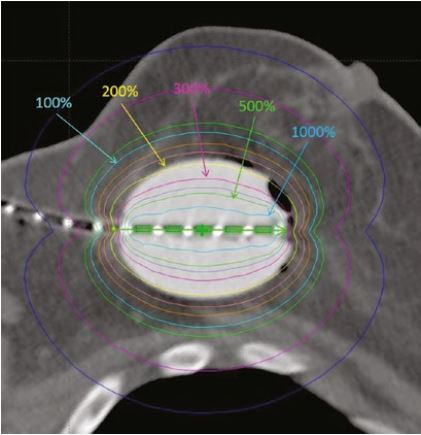
\includegraphics[width=0.5\textwidth]{Imagens/falloffDoseMammosite.JPG}
			\caption{Distribuição de dose com um balão de mama inflado. A dose de prescrição está a 1 cm de profundidade da superfície do balão. Caso o balão seja esvaziado, a dose nesse mesmo ponto pode ficar 10 vezes maior que a dose de prescrição.}
			\label{img:DistribuicaoDoseBalao}
		\end{figure}

		São 3 fatores que impactam na forma da distribuição de dose em braquiterapia: \textbf{\textcolor{CarnationPink}{distância da fonte, forma e encapsulamento e o material do encapsulamento}}.

		\begin{enumerate}
			\item Para distâncias grandes da fonte, ou seja, para distâncias de no mínimo duas vezes o tamanho da fonte, a distribuição de dose é governada pela \textbf{\textcolor{CarnationPink}{lei do inverso quadrado}}. Porém, quanto mais próximo está o ponto de análise da fonte, menos aplicável é a lei do inverso quadrado.
			
			\item A forma cilíndrica da fonte faz com que a dose ao longo do seu eixo longitudinal seja diminuída devido à penetração em uma maior quantidade de material quando comparado ao eixo axial, causando uma maior filtração da radiação nessa direção. A    \ref{img:distribuicaoDeDose} mostra o comportamento da distribuição de dose ao longo do eixo longitudinal da fonte.
			
				\begin{figure}[h]
					\centering
					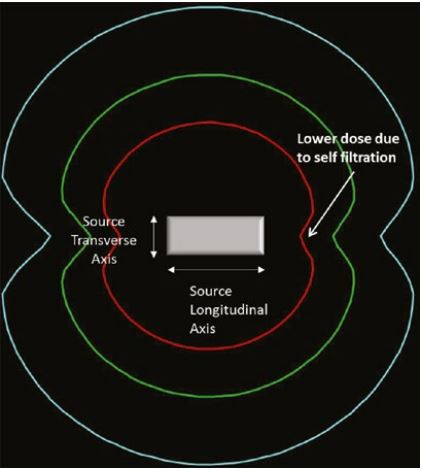
\includegraphics[width=0.5\textwidth]{Imagens/distribuicaoDeDose.JPG}
					\caption{Distribuição de dose na água para uma fonte realística de $\mathrm{{}^{192}Ir}$}
					\label{img:distribuicaoDeDose}
				\end{figure}

			\item O material do encapsulamento está diretamente relacionado à absorção e ao espalhamento dos fótons causando uma atenuação dos fótons emitidos.
		\end{enumerate}
	
	\section{Métodos de Cálculo de Dose}

		Existem diferentes métodos para obtenção da Dose envolvida em procedimentos de braquiterapia. 

		\subsection{Cálculos de Dose Cumulativa}

			São utilizados para determinar a dose total entregue ao longo de todo o período de tratamento. Como a atividade muda com o decorrer do tempo, a taxa de dose também muda com o decorrer do tempo e pode ser obtida através da seguinte relação:

				\begin{equation}
					\dot{D}(t) = \dot{D_0} e^{-\lambda t}
					\label{eq:taxaDeDose}
				\end{equation}

			onde,

			$\dot{D_0}$ é a taxa de dose inicial da amostra.

			A dose total acumulada em um tempo específico pode ser obtida integrando a   \ref{eq:taxaDeDose} no tempo t, ou seja:

				\begin{equation}
					D(t) = \int_{t_0}^{t} \dot{D_0} e^{-\lambda t}\,dt
					\label{eq:integralDaDose}
				\end{equation}

			Resolvendo a integral apresentada na   \ref{eq:integralDaDose}, obtemos a relação que nos fornece a dose acumulada após um tempo t (dose total).

				\begin{equation}
					D(t) = \frac{1}{\lambda} \; \dot{D_0} \; (1 - e^{-\lambda t})
					\label{eq:doseCumulativa}
				\end{equation}

			Sabendo que $$\frac{1}{\lambda} = \tau = 1.44 t_{1/2}$$ A   \ref{eq:doseCumulativa} pode ser escrita da forma:

				\begin{equation}
					D(t) = 1.44\,t_{1/2} \,\dot{D_0} (1 - e^{-\lambda t})
				\end{equation}

			No caso de implantes permanentes cuja meia vida do elemento é curta, o tempo de tratamento será muito maior que o tempo de meia vida deste elemento pois a dose será entregue ao longo de toda a vida da fonte. Podemos fazer então uma aproximação na   \ref{eq:doseCumulativa} quando $t >> t_{1/2}$: 

			Como $$t >> t_{1/2}$$ então $$\frac{t}{t_{1/2}} >> 1$$

			Como $$\lambda = \frac{ln 2}{t_{1/2}}$$ Substituindo este valor na   \ref{eq:doseCumulativa} temos que: 

			$$ D(t) = \frac{1}{\lambda}  \; \dot{D_0} \; \left(1 - e^{-\frac{ln 2}{t_{1/2}} t}\right) $$

			$$D(t) = \frac{1}{\lambda}  \; \dot{D_0} \; \left(1 - \frac{1}{e^{ln 2 \frac{t}{t_{1/2}}}}\right)$$

			Avaliando no limite quando $\frac{t}{t_{1/2}} \rightarrow \infty$ temos:

			$$ \lim_{{\frac{t}{t_{1/2}}} \to \infty} D(t) = \lim_{{\frac{t}{t_{1/2}}} \to \infty} \frac{1}{\lambda}  \; \dot{D_0} \; \left(1 - \frac{1}{e^{ln 2 \frac{t}{t_{1/2}}}}\right)$$

			Aplicando as propriedades de limite temos

			$$\lim_{{\frac{t}{t_{1/2}}} \to \infty} D(t) = \frac{1}{\lambda} \; \dot{D_0} \;  \left(\lim_{{\frac{t}{t_{1/2}}} \to \infty} 1 - \lim_{{\frac{t}{t_{1/2}}} \to \infty} \frac{1}{e^{ln 2 \frac{t}{t_{1/2}}}}\right)$$

			Como $1/ \lambda$ e $\dot{D_0}$ são constantes e:

			$$\lim_{{\frac{t}{t_{1/2}}} \to \infty} 1 = 1$$

			$$\lim_{{\frac{t}{t_{1/2}}} \to \infty} \frac{1}{e^{ln 2 \frac{t}{t_{1/2}}}} = \frac{1}{e^{\infty}} = 0 $$

			Chegamos na   de dose total quando $t >> t_{1/2}$:

			\begin{equation}
				D = \frac{1}{\lambda} \; \dot{D_0} = \tau \; \dot{D_0} = 1.44 \; t_{1/2} \; \dot{D_0}
				\label{eq:aproximacaoImplantesPermanentes}
			\end{equation}


			Outro caso a ser avaliado, são em implantes temporários cujo tempo de exposição é muito menor que o tempo de meia vida da fonte radioativa. Podemos fazer então uma aproximação da dose total para os casos em que $t << t_{1/2}$. 


			Como $t << t_{1/2}$, então

			$$\frac{t}{t_{1/2}} << 0 $$

			Podemos então utilizar a série de taylor para expandir o termo da exponencial. 

			Para $x << 0$

			$$e^x = 1 + x + \frac{x^2}{2!} + \frac{x^3}{3!} + \dots$$

			Truncando a série na primeira ordem, pois os termos quadráticos são ínfimos, temos que

			$$ e^{-ln 2 \frac{t}{t_{1/2}}} = 1 - ln 2 \; \frac{t}{t_{1/2}}$$

			Substituindo na   \ref{eq:doseCumulativa} temos então

			$$D(t) = \frac{1}{\lambda} \; \dot{D_0} \; \left[1 - \left(1 - \ln 2 \; \frac{t}{t_1/2}\right)\right]$$

			Fazendo as devidas simplificações, chegamos na   para a dose total quando $t << t_{1/2}$

			\begin{equation}
				D(t) = \dot{D_0} \; t
				\label{eq:AproximacaoImplantesTemporarios}
			\end{equation}

			Portanto a Dose total é dada pela multiplicação da taxa de dose inicial pelo o tempo de tratamento, o que faz sentido pois a atividade de uma fonte com o tempo de meia-vida muito maior que o tempo de tratamento, não sofrerá mudanças significativas nesse curto espaço de tempo.


			Nos casos em que o tempo de tratamento é da ordem do tempo de meia vida da fonte, haverá uma mudança significativa da Atividade durante o tempo de tratamento, então a dose total é obtida através da   \ref{eq:doseCumulativa}.

		\subsection{Método de Integral e Interpolação}

			Foram métodos historicamente utilizados para os cálculos de dose em fontes com formatos tubulares ou na forma de sementes.

			O método \textbf{\textcolor{CarnationPink}{Integral de Sievert}} subdivide a fonte em n partes iguais. As partes são divididas em partes pequenas o suficiente de forma que possam ser aproximadas para fontes pontuais. Para um determinado ponto próximo à fonte, a dose é determinada somando às contribuições das n partes considerando os fatores de correção aplicados separadamente para cada parte. Os fatores de correção utilizados são: \textit{fator distância, filtração oblíqua, atenuação e espalhamento}.

			O \textbf{\textcolor{CarnationPink}{Método de Interpolação}} utiliza tabelas de dados de conjuntos de pontos que foram previamente obtidos através de técnicas experimentais ou de modelos teóricos. As tabelas \textit{\textcolor{CarnationPink}{along-and-away}} foram muito utilizadas para tratamentos com $\mathrm{{}^{137}Cs}$ e dados tabelados também foram muito utilizados nos sistemas Paterson-Parker e Quimbly.

		\subsection{Formalismo Modular: TG-43}

			É o método padrão para cálculos de taxa de dose 1D e 2D. Este método assume uma fonte cilíndrica simétrica, considerando as diferenças na distribuição de dose causadas pela forma da fonte. A dose obtida nesse formalismo é determinada para um meio homogêneo de água e portanto não considera a heterogeneidade de um meio não-homogêneo. Os dados tabelados deste formalismo foram obtidos através de medidas experimentais e através de simulações de Monte-Carlo para fontes conhecidas, e são utilizados nos sistemas de planejamento.

			Este método é dividido em módulos onde cada parâmetro depende da posição do ponto de cálculo de dose com respeito à fonte. A    \ref{img:FormalismoTg43} mostra a geometria utilizada para cálculo da distribuição de dose. A posição do ponto de cálculo é dada em coordenadas polares $\mathrm{P(r, \theta)}$ onde $r$ é a distância radial do ponto até o centro da fonte e $\theta$ é o ângulo formado com o eixo longitudinal da fonte (eixo z na   ) tomado a partir centro da fonte. A posição $\mathrm{P_0(r_0, \theta_0)}$ é a posição de referência dos cálculos localizada radialmente a 1 cm da fonte ($r_0 = 1 \; cm$) ao longo do eixo central da fonte (eixo y na   ) fazendo um ângulo $\theta_0 = \pi / 2$ com o eixo longitudinal da fonte.


				\begin{figure}[h]
					\centering
					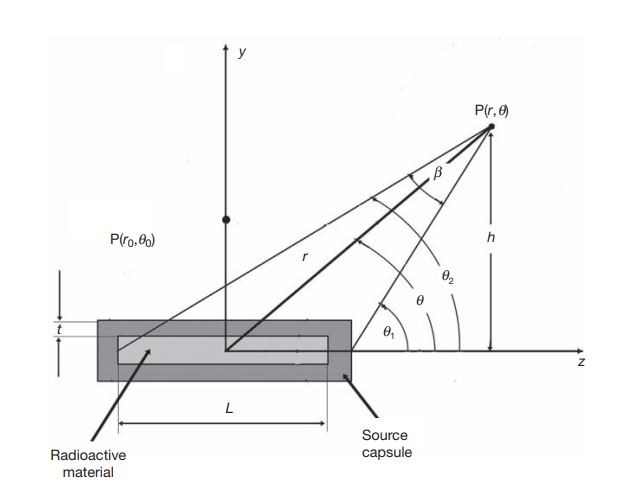
\includegraphics[width=0.8\textwidth]{Imagens/esquemaFormalismoTg43.JPG}
					\caption{Geometria Utilizada para determinação da taxa de dose no Formalismo do TG 43}
					\label{img:FormalismoTg43}
				\end{figure}

			A taxa de dose em função da posição do ponto de cálculo é dada por:

			\begin{equation}
				\dot{D}(r, \theta) = S_k \; \varLambda \; \frac{G(r, \theta)}{G(r_0, \theta_0)} 
				\; g(r) \; F(r, \theta)
				\label{eq:formalismoTg43}
			\end{equation}

			onde:

			\begin{itemize}
				\item \textbf{\textcolor{CarnationPink}{$\varLambda$} : } é a constante de taxa de dose responsável por corrigir a medida no ar para a água. É definida como a taxa de dose na água por unidade de força Kerma-ar na posição de referência $\mathrm{P_0(r_0, \theta_0)}$. Esta constante faz com que o cálculo de dose seja feito para um meio homogêneo de água, o que é mais adequado para simular um paciente, mesmo não considerando a heterogeneidade e não no ar, como é definida a força kerma-ar.

					\begin{equation}
						\varLambda = \frac{\dot{D}(r_0, \theta_0)}{S_k}
					\end{equation}

					$$[\varLambda] = cGy / U \cdot h$$

				\item \textbf{\textcolor{CarnationPink}{$S_k$} : } É a força Kerma-ar. É definida como a taxa kerma-ar medida no ar livre em uma distância específica do centro da fonte ao longo do seu eixo transversal multiplicado pelo quadrado da distância do ponto à fonte.

					\begin{equation}
						S_k = \dot{K}(d) \cdot d^2
					\end{equation}

					$$[S_k] = U = cGy \cdot cm^2 / h$$

				\item \textbf{\textcolor{CarnationPink}{$G(r, \theta)$}: } É a função Geométrica. Fornece a efetiva lei do inverso quadrado pois considera a variação da dose relativa devido à distribuição espacial da atividade dentro da fonte (forma da fonte). Depende apenas da distância radial e angular do ponto de análise portanto não considera o espalhamento e a atenuação da fonte. Em outras palavras, A função geométrica reflete a queda de dose com base na lei do inverso quadrado para a geometria da fonte.
				
					$$[G(r_ \theta)] = cm^{-2}$$

					Para uma fonte Pontual:

					\begin{equation}
						G(r, \theta) = \frac{1}{r_2}
					\end{equation}

					Para uma fonte cilíndrica:

					\begin{equation}
						G(r, \theta) = \frac{\beta}{L \; r \; sen(\theta)}, \qquad para \qquad \theta \neq 0
					\end{equation}

					\begin{equation}
						G(r, \theta) = \left(r^2 - \frac{L^2}{4}\right)^{-1}, \qquad para \qquad \theta = 0
					\end{equation}
				
				\item \textbf{\textcolor{CarnationPink}{$g(r)$} : } É chamada de Função de dose radial. É uma quantidade adimensional que considera o falloff da dose ao longo do plano transversal da fonte devido ao espalhamento e a atenuação no material do encapsulamento da fonte e devido a alteração do meio de ar para a água. É definida ao longo do eixo transversal $\mathrm{(\theta = \pi / 2)}$, portanto depende apenas da distância radial do ponto à fonte. Em outras palavras, a função de dose radial reflete na queda da dose devido ao espelhamento e atenuação da radiação onde o espalhamento aumenta a dose na profundidade e a atenuação diminui a dose na profundidade. Seus valores são tabelados e podem ser encontrados no update do TG-143 e em seu suplemento.
				
					Na distância de referência $r_0$

					$$g(r_0) = 1$$
				
				\item \textbf{\textcolor{CarnationPink}{$F(r, \theta)$} : } É chamada de Função de Anisotropia. Leva em consideração o formato anisotrópico da distribuição de dose causado pela própria filtração do encapsulamento da fonte e a transmissão oblíqua através do encapsulamento. Fornece a distribuição de dose para ângulos diferentes de $\theta = \pi / 2$, ou seja, para pontos em ângulos fora do eixo transversal da fonte. Em outras palavras, a função de anisotropia fornece a variação da dose em função do ângulo polar formado com o plano transversal da fonte.
				
					Para $\theta = \theta_0 = \pi/2$

					$$F(r, \theta_0) = 1$$

			\end{itemize}
			
			Ao aplicar a   \ref{eq:formalismoTg43} para uma \textbf{\textcolor{CarnationPink}{fonte pontual}}, pode-se desconsiderar a anisotropia da distribuição de dose em função do ângulo,  pois a distribuição de dose para uma fonte pontual é isotrópica na mesma distância radial. Nesses casos, não se considera a posição angular do ponto de cálculo, passando a depender apenas da posição radial. Portanto a função de anisotropia passa ser: $F(r, \theta) \rightarrow \Phi (r)$,  que é um fator de anisotropia 1D dado pela média da taxa de dose em cada distância em relação ao ângulo sólido.
			
			\begin{equation}
				\dot{D}(r) = S_k \; \varLambda \; \left(\frac{r_0}{r} \right)^2 \; g(r) \; \Phi (r)
				\label{eq:aproxModularFontePontual}
			\end{equation}
			
			A Aproximação fornecida pela   \ref{eq:aproxModularFontePontual} pode ser aplicada sempre que:

			\begin{enumerate}
				\item A distância do ponto até a fonte é de no mínimo duas vezes o tamanho efetivo da fonte de modo que a forma da distribuição de dose nesse ponto não cause impacto no cálculo da dose.
				\item Quando as fontes estão distribuídas aleatoriamente de forma que é tomada uma média dos efeitos de anisotropia.
			\end{enumerate}

			Tratamentos de próstata com LDR são um exemplo de aproximação para fonte pontual enquanto que os tratamentos HDR utilizam o formalismo em si para as fontes cilíndricas.

		\subsection*{\textcolor{CarnationPink}{Exemplo: Tratamento de Próstata com fontes de Baixa Energia}}

			É comum ser realizado um planejamento intra-operatório para implantes de próstata onde é adquirida uma imagem de ultrasonografia transretal, que é transferida para o sistema de planejamento. Na imagem são delineados o volume alvo, o reto e a uretra. Normalmente o sistema de planejamento assumo os cálculos de distribuição de dose para uma fonte pontual. Modelos de fontes lineares podem ser utilizados desde que parta do pressuposto que essas fontes são paralelas às agulhas, porém essa forma pode levar à imprecisões nos cálculos de dose. Por outro lado, a orientação das fontes podem ser mais precisamente definidas utilizando uma imagem de Tomografia Computadorizada (TC) durante a avaliação da dose pós-implante através de métodos de segmentação automatizados. Nestes casos a distribuição de dose pode ser calculada através da soma da dose de cada semente.

			\begin{enumerate}
				\item \textbf{As sementes do modelo Amersham 6702 de \textsuperscript{125}I são utilizadas em um implante de próstata. A força Kerma-ar para estas sementes é de 0.5 U. Uma semente está a 3.0 cm da parede anterior do reto.}
				
					\begin{enumerate}
						\item \textbf{Qual é a taxa de dose dessa semente até o ponto mais próximo do reto?}
						\item \textbf{Quanta dose este ponto receberá da fonte após 1 mês?}
						\item \textbf{Qual a dose total que será recebida devido à esta fonte?}
					\end{enumerate}
			\end{enumerate}

			\textbf{\textcolor{CarnationPink}{Solução:}}

			\begin{quote}
				\color{MediumOrchid}
				A dose neste caso deve ser avaliada utilizando a aproximação para uma fonte pontual pois embora a dose seja calculada para apenas uma semente, o ponto de análise está a uma distância superior a 2 vezes o tamanho da fonte. De acordo com o TG-43, este modelo de fonte possui comprimento L = 3.0 mm.

				Os valores das quantidades necessárias para determinação da dose foram obtidos no update do TG-43 e todos os dados necessários para os cálculos podem ser conferidos na tabela \ref{tb:paramExercCalcDose}:

				\begin{table}[h]
					\color{MediumOrchid}
					\centering
					\captionsetup{labelfont={color=MediumOrchid, bf}}
					\caption{\textcolor{MediumOrchid}{Valores dos parâmetros necessários para a resolução do exercício.}}
					\label{tb:paramExercCalcDose}
					\begin{tabular}{c c}
					\hline
					\multicolumn{2}{c}{Valores para r = 3.0 cm } \\
					\multicolumn{2}{c}{considerando uma fonte pontual} \\
					\midrule[1.5pt]
					Parâmetro & Valor \\
					\addlinespace[4pt]
					\midrule[1.5pt]
					$S_k$ & $0.5 \; U$ \\
					\addlinespace[4pt]
					\hline
					$\varLambda$ & $1.036 \; cGy  \cdot h^{-1} \cdot U^{-1}$ \\
					\addlinespace[4pt]
					\hline
					$g_p(r)$ & $0.702$ \\
					\addlinespace[4pt]
					\hline
					$\phi_{an}(r)$ & $0.951$ \\
					\addlinespace[4pt]
					\hline
					\multirow{2}{*}{$t_{1/2}$} & $59.4 \; dias$\\
					 & $1425.6 h$ \\
					\addlinespace[4pt]
					\hline
					 $r_0$ & $ 1 \; cm$ \\
					\addlinespace[4pt]
					\hline
					\hline
					
					\end{tabular}
				\end{table}

				\textbf{(a)} A taxa de dose  no ponto é então:

					$$\dot{D}(r) = S_k \cdot \varLambda \cdot \left(\frac{r_0}{r}\right)^2 \cdot g(r) \cdot \phi_{an}(r)$$
				
					Fazendo as devidas substituições temos:

					$$\dot{D}(r= 3cm) = 0.5 \cdot 1.036 \cdot \left(\frac{1}{3}\right)^2 \cdot 0.702 \cdot 0.951$$

					Portanto, temos que

					$$\dot{D}(r= 3cm) = 0.0384 \; cGy / h$$

				\textbf{(b)} A dose acumulada após 1 mês de implante devido à fonte pode ser obtida através da  :

					$$D(t) = \dot{D_0} \cdot 1.44 \cdot t_{1/2} \cdot \left(1 - e^{- ln 2 \cdot \frac{t}{t_{1/2}}}\right)$$

					Sendo $t = 30 \; dias$, e utilizando a taxa de dose inicial obtida no item (a), temos então que:

					$$D(t = 30 \; dias) = 0.0384 \cdot 1.44 \cdot 1425.6 \cdot \left(1 - e^{- 0.693 \cdot \frac{30}{59.4}}\right) $$

					Portanto, a dose após 1 mês de implante é:

					$$D(t = 30 \; dias) = 23.28 \; cGy$$

					\textbf{\textcolor{CarnationPink}{Obs:}} \textit{O valor da meia vida dentro da exponencial foi utilizado em dias para ficar da mesma dimensão do tempo de implante; Fora da exponencial foi utilizado em horas para obter a dose em Gy uma vez que a taxa de dose foi determinada em Gy/h, caso contrário essa conversão deveria ter sido feita no final do exercício.}

				\textbf{(c)} A dose total para um implante permanente cuja meia vida é muito menor que o tempo do implante é obtida através da relação:

					$$D = 1.44 \cdot \dot{D_0} \cdot t_{1/2}$$

					Portanto a dose total recebida no ponto devido a esta fonte será de:

					$$D = 1.44 \cdot 0.0384 \cdot 1425.6$$
					$$D = 78.83 \; cGy$$

				\textbf{\textcolor{CarnationPink}{Obs:}} \textit{ A dose no ponto foi calculada para a contribuição de apenas 1 semente. Para obter a dose total recebida nesse ponto deve-se somar a contribuição de todas as fontes inseridas no implante.}



			\end{quote}

		
		\subsection{Sistemas Clássicos para Implantes Intersticiais}

			Antes da era computacional, eram utilizadas tabelas pré-calculadas para determinar a quantidade de rádio necessária em um \textit{\textbf{\textcolor{CarnationPink}{Implante Intersticial}}}.

			\begin{figure}[h]
				\centering
				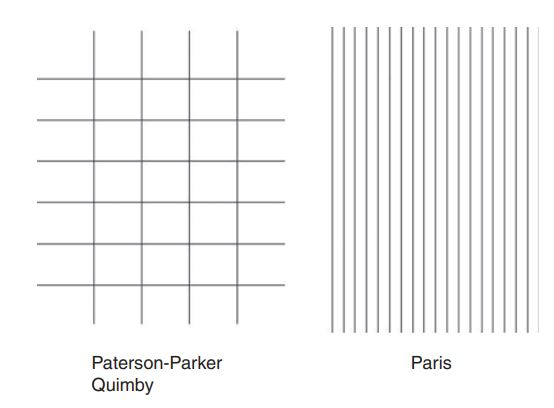
\includegraphics[width=0.7\textwidth]{Imagens/carregamentosHistoricos.JPG}
				\caption{Sistemas de Carregamento Clássicos}
				\label{img:carregamentosHistoricos}
			\end{figure}


			\begin{itemize}
				\item Sistema Manchester (Paterson-Parker): Utilizavam agulhas ou cateteres perpendiculares entre si (crossed ends), como mostra a    \ref{img:carregamentosHistoricos}.  Este sistema possui diferentes tabelas de carregamento de dose para um único plano, dois planos e implantes volumétricos. Utilizava o carregamento não uniforme periférico gerando uma distribuição de dose homogênea.
				
				\item Sistema Quimbly: Utilizavam agulhas ou cateteres perpendiculares entre si, semelhantemente ao sistema Manchester; A principal diferença entre esses sistemas é que no Quimbly utilizava o carregamento uniforme gerando uma distribuição de dose com um ponto quente central no volume implantado. 
				
				\item Sistema Paris: utilizava implantes volumétricos com multiplas agulhas ou cateteres paralelos entre si. Onde as agulhas eram distribuidas igualmente espaçadas entre si e com carregamento uniforme das fontes, gerando um ponto quente central. 
			\end{itemize}

% TODO: Sistema Classico Fletcher

		\subsection{Cálculos de Dose Baseados em Imagens}

			Algoritmos de cálculo de dose baseados em modelos podem ser utilizados para cálculos de distribuição de dose levando em consideração um meio heterogêneo, uma vez que o formalismo do TG-43 considera o meio homogêneo em seus cálculos.
			
			Os algoritmos de cálculo consideram o impacto de diferentes meios materiais na dispersão da dose através de:

				\begin{itemize}
					\item Simulação e Acoplamento do par fóton-elétron no transporte de radiação; ou
					\item Através da utilização de técnicas de integração da dispersão multidimensional.
				\end{itemize}
			
			Os métodos de cálculos computacionais mais utilizados são:

				\begin{itemize}
					\item \textbf{\textit{\textcolor{CarnationPink}{Collapsed Cone Convolution-Superposition}}}, que utilizam Kernels para calcular a dose de radiação do feixe primário e do feixe espalhado no qual mapeia, espacialmente, a disposição de energia no meio. \textit{Exemplo:} \textit{\textbf{Oncentra\textsuperscript{\textregistered}}, Sistema de planejamento de braquiterapia da Elekta que implementa o algoritmo Convolution-Superposition}.
					
					\item \textbf{\textit{\textcolor{CarnationPink}{Grid-based Boltzmann Solvers}}}, onde é utilizada uma abordagem determinística para resolver diretamente a   de transporte linear de Boltzmann. \textit{Exemplo:} \textit{\textbf{Acuros\textsuperscript{\textregistered}}, algoritmo implementado no sistema de planejamento Brachyvision\textsuperscript{\textregistered} da Varian}.
					
					\item \textbf{\textit{\textcolor{CarnationPink}{Monte Carlo Simulations}}}, que utiliza abordagens estocásticas para resolver a   de transporte linear de Boltzmann através de amostragens aleatórias. É um modelo mais presente em pesquisas científicas.
					
					\end{itemize}
		
	\section{Braquiterapia de Baixa Energia}
		

		Fontes consideradas de baixa energia são aquelas que emitem fótons com energia da ordem de 50 KeV, como o \textsuperscript{125}I, \textsuperscript{103}Pd e \textsuperscript{131}Cs.

		Devido a baixa energia dos fótons emitidos por estas fontes, a proteção radiológica se torna mais efetiva por dois motivos:

			\begin{enumerate}
				\item O feixe é atenuado pelo próprio paciente, nos casos de implantes permanentes.
				\item A blindagem de chumbo necessária para estas fontes é mínima nos casos de implantes temporários, como ocorre em placas oftalmológicas.
			\end{enumerate}
		
		As principais aplicações de fontes de braquiterapia de baixa energia são feitas nos implantes permanentes de próstata guiados por ultrasonografia transretal. Embora tenha uma aplicação mais limitada, também podem ser aplicadas no tratamento de melanomas intraoculares e tumores pulmonares em estágio inicial.

		Quando uma fonte é considerada como \textit{\textcolor{CarnationPink}{rádio-equivalente}}, como ocorre com as fontes de \textsuperscript{137}Cs, \textsuperscript{60}Co e \textsuperscript{198}Au, seu espectro é governado por raios-$\mathrm{\gamma}$ de alta energia e podem facilmente ser especificadas em termos da definição ``\textit{miligramas de rádio equivalente}", possuindo métodos mais simples para cálculos de dose, pois a energia desses fótons é minimamente modificada pela construção da fonte e pela atenuação no tecido. 

		Porém, quando se trata de fontes de baixa energia, como o \textsuperscript{125}I, \textsuperscript{103}Pd e o \textsuperscript{131}Cs, os cálculos de dose já não são tão simples uma vez que a energia do feixe é significativamente modificada devido à atenuação e ao espalhamento dos fótons de baixa energia causados pelo encapsulamento da fonte. Para estes casos é necessária uma modificação apropriada no formalismo de cálculo para a determinação da calibração da força da fonte.

		\subsection{Design e construção das Sementes}

			O formalismo de cálculo estabelecido pelo TG-43 contemplava primordialmente os modelos de sementes:

				\begin{itemize}
					\item \textsuperscript{125}I: Nycomed-Armsham 6702 e 6711
					\item \textsuperscript{103}Pd: Theragenics TP-200
					\item  \textsuperscript{192}Ir: Best Medial e Alpha-Omega
				\end{itemize}
			
			O Report Tg-43 foi atualizado para corrigir inconsistências no report original e para incluir recomendações a cerca de fontes de braquiterapia de baixa energia, incluindo conjuntos de dados dosimétricos paras as novas fontes de \textsuperscript{125}I e \textsuperscript{103}Pd além dos guidelines para a determinação dos parâmetros dosimétricos das fontes de baixa energia.


			As fontes desenvolvidas possuem normalmente uma dimensão externa de 4.5 mm de comprimento e 0.8 mm de diâmetro, onde:

				\begin{itemize}
					\item O diâmetro é estabelecido sendo o mesmo diâmetro do calibre de uma agulha utilizada na braquiterapia Intersticial; E
					\item O tamanho é definido com base na regulamentação dos EUA para materiais radioativos sob a forma especial com limite de 0.5 cm para fins de embalagem e envio.
				\end{itemize}

				As características básicas de uma fonte são:

				\begin{enumerate}
					\item Possuem um encapsulamento da fonte que deve ser feito através de uma cápsula de Titânio, sendo normalmente um tubo fino fabricado pelo processo de extrusão.
					\item Possuem envólucros de extremidades que devem ser na forma de soldas de extremidade, copos ou outros mecanismos afim de vedar os tubos de titânio após os componentes internos serem inseridos.
					\item Possuem portadores de fonte ativa que devem estar na forma de esferas ou cilindros.
					\item Possuem um material com a fonte ativa contendo o material radioativo incorporado ao portador da fonte.
				\end{enumerate}


			Em uma fonte ideal, espera-se que a distribuição de dose em volta da fonte seja uniforme e que haja uma reprodutibilidade na distribuição de dose inter-fontes. Portanto, algumas características dosimétricas podem ser afetadas devido à problemas na fabricação da fonte e portanto durante a fabricação de uma fonte deve-se atentar as seguintes características:

				\begin{enumerate}
					\item O encapsulamento da fonte deve conter uma espessura uniforme de titânio, o que é possível ser alcançado através de equipamentos de modelagem mais sofisticados.
					
					\item O projeto dos envólucros de fechamento devem ser finos e uniformes e devem garantir uma variação mínima inter-sementes. 

						\textit{Envólucros de fechamentos mais espessos, como soldas ou copos, podem aumentar a anisotropia na distribuição de dose próximo às extremidades da semente, reduzindo a precisão do cálculo da dose baseado em fontes pontuais. Variações na espessura da solda entre as sementes causam desvios nos cálculos. Essas variações, embora clinicamente insignificantes, tem o potencial de aumentar significativamente as incertezas dos valores calculados da função de anisotropia da fonte devido às incertezas nas espessuras médias das soldas de fechamento utilizada nos cálculos. Além disso, pode também aumentar a incerteza nos valores medidos de anisotropia}
					
					\item A geometria e o material dos portadores de fonte ativa podem afetar as características dosimétricas da fonte:
					
						\begin{enumerate}
							\item Utilizando \textbf{Prata} como o material do portador de fonte ativa, os raios-x da camada K desse material possuem energia de 25.51 KeV; Portanto a prata irá suavizar o espectro de energia do fotón emitido pela fonte encapsulada. Isso resulta em uma menor constante de taxa de dose em sementes de \textsuperscript{125}I com portador de prata quando comparado aos outros materiais de portadores de fonte.
							
								\textit{\textcolor{CarnationPink}{Exemplo:}} 
									\begin{itemize}
										\item Valor médio da constante de taxa de dose para o \textsuperscript{125}I encapsulado com Ag:
										
											\textbf{$\mathrm{0.953 \; cGy \cdot h^{-1} \cdot \; U^{-1}}$}
										\item Valor médio da constante de taxa de dose para outras sementes de \textsuperscript{125}I:
										
											\textbf{$\mathrm{1.026 \; cGy \cdot h^{-1} \cdot \; U^{-1}}$}
									\end{itemize}

							\item A falta de reprodutibilidade do posicionamento dos portadores da fonte dentro do encapsulamento de titânio pode afetar negativamente a precisão nas medidas da distribuição de dose em volta da fonte, semelhantemente ao que ocorre com as diferenças das espessuras da solda no fechamento da semente em sua parte interna.
							
						\end{enumerate}
					
					\item A falta de uniformidade na deposição do material da fonte radioativa nos carregadores da fonte podem aumentar os valores calculados e medidos da anisotropia da distribuição de dose e até mesmo da função de dose radial.
					
				\end{enumerate}

			As incertezas na distribuição de dose devido à fabricação da fonte são reduzidas conforme tenha um aumento do número de fontes utilizadas no tratamento do paciente; Além dessa incertezas serem mais enunciadas à curtas distâncias da fonte. Pode-se afirmar então que os cálculos de dose baseados em fontes pontuais permitem precisão adequada do cálculo da dose pois são tomados à uma distância segura da fonte ou devido à contribuição de várias fontes, situações onde os erros de fabricação são desprezíveis.

			Nenhuma alteração na fabricação da fonte deve ser feita sem comunicação prévia devido a alta sensibilidade das fontes de baixa energia o que faz com que qualquer alteração pode levar a um impacto dosimétrico.

		\subsection{Dosimetria das Fontes de Baixa Energia}

			As fontes de braquiterapia são descritas com base em sua atividade aparente. A atividade aparente é obtida através da taxa de exposição na distância de calibração em um laboratório acreditado. Com bases nesses valores que foram calculados as distribuições de dose 2-D.

			O padrão para determinar a força da fonte é a \textbf{\textcolor{CarnationPink}{Força Kerma-AR}}, que pode ser convertida para a taxa de exposição à 1m da fonte através da relação:

				\begin{equation}
					S_k = \dot{X}(R \cdot h^{-1}) \cdot 0.876 \; (cGy/R) \cdot (1 \; m)^2
				\end{equation}
			
			A força Kerma-ar é definida como o produto da força Kerma-ar devido aos fótons de energia $\dot{K}$ maiores que a energia de corte $\delta$ a uma distância $d$ e o quadrado da distância:

				\begin{equation}
					S_k = \dot{K}_\delta (d) \cdot d^2
				\end{equation}

				\textbf{\textcolor{CarnationPink}{Obs:} } O valor valor para energia de corte para fótons de baixa energia é de:

				$$\delta = 5 \; \; KeV$$
				
			A força Kerma-ar em uma fonte cilíndrica pode ser calibrada através de comparação direta com uma fonte do mesmo tipo calibrada no laboratório acreditado.

			\textbf{\textcolor{CarnationPink}{Obs:}} O NIST é um laboratório acreditado onde a calibração é feita com uma câmara de ar livre com ampla angulação (incidência de vários ângulos) com uma aproximação de $0.01 \; \; Gy \; m^2 \; h^{-1}$. É feita uma filtragem com alumínio para excluir a contaminação com fótons de baixa energia da ordem da energia de corte na definição da Força Kerma-ar para minimizar a incerteza na medição.

			A dose 2-D é então determinada pela   \ref{eq:formalismoTg43} levando em consideração a correção feita na exposição para determinar a força kerma-ar;

		\subsection{Aplicações Clínicas dos Fótons de Baixa Energia}

			Os raios-X de baixa energia possuem maior Transferência Linear de Energia \textbf{\textcolor{CarnationPink}{(LET)}} quando comparados aos raios-x de alta energia. Isto resulta em uma maior Efetividade Biológica Relativa \textbf{\textcolor{CarnationPink}{(RBE)}}, o que é uma vantagem na morte tumoral.

			As energias típicas para braquiterapia de baixa energia estão abaixo de 50 KeV, com energias efetivas semelhante aos raiox-X de baixa energia entre 30KeV e 150 KeV. No caso do \textsuperscript{125}I, a RBE comparada ao \textsuperscript{60}Co varia entre 1.1 - 2.0. Já o \textsuperscript{103}Pd possui um valor de LET ligeiramente maior que o \textsuperscript{125}I e seus valores de RBE são aceitos como sendo aproximadamente 10\% mais altos.

			Os valores da RBE também dependem da dose e da taxa de dose que serão entregues. Esses valores são determinados principalmente pela natureza e duração do implante. A tabela \ref{tb:rbeI25} mostra a diferença dos valores de RBE em relação ao \textsuperscript{60}Co com base no tipo de implante.

				\begin{itemize}
					\item Em casos de \textcolor{CarnationPink}{Implantes Temporários}, a dose típica a ser entregue varia entre 60 Gy - 90 Gy em poucos dias de tratamento a uma taxa de dose variandro ente 0.5 Gy/h até 0.8 Gy/h utilizando sementes com alta atividade.
					\item Já nos casos de \textcolor{CarnationPink}{implantes permanentes}, a taxa de dose timicamente utilizada é menor que 0.2 Gy/h utilizando sementes de baixa atividade.
				\end{itemize}

				\begin{table}[h]
					\centering
					\caption{Valores de RBE para o \textsuperscript{125}I}
					\label{tb:rbeI25}
					\begin{tabular}{c c}
					\toprule
					Técnica & RBE \\
					\midrule[1.5pt]
					Implantes Temporários & 1.15 - 1.20 \\
					Implantes Permanentes & $>$ 2.0 \\
					\bottomrule
					\bottomrule
					\end{tabular}
				\end{table}

			Sendo $\lambda$ a constante de decaimento, $\mu$ a constante de recuperação do dano sub-letal e $T$ o tempo de duração de uma seção de braquiterapia, podemos extrair as seguintes relações:
			
			\begin{itemize}
		
			
				\item A dose para os implantes temporários pode ser obtida através da   \ref{eq:doseCumulativa}. 

					$$D(t) = \frac{1}{\lambda} \cdot \dot{D_0} \cdot \left(1 - e^{-\lambda t}\right)$$

				\item A dose biológicamente eficaz \textbf{\textcolor{CarnationPink}{(BED)}} para implantes temporários pode ser obtida através da  :

					\begin{equation}
						BED = \frac{1}{\lambda} \dot{D_0}\left(1 - e^{-\lambda t}\right)
						\left\{ 1 + \frac{2 \dot{D_0}\lambda}{(\mu - \lambda)(\alpha / \beta) (1 - e^{-\lambda t})}
						\left[\frac{1}{2\lambda}(1 - e^{-\lambda t }) - \frac{1}{\mu + \lambda} (e - e^{-(\mu + \lambda) t})\right]\right\} 
					\end{equation}

				\item O BED para uma duração T da seção de braquiterapia é obtido através da relação:

					\begin{equation}
						BED_{BT} = D \left\{ 1 + \frac{2 \cdot D}{(\alpha / \beta)\mu \cdot T}
						\left[1 - \frac{1}{\mu T} (1 - e^{-\mu T})\right]\right\}
					\end{equation}
				
				\item A Dose Total para implantes permanentes é dada por:
					
					\begin{equation}
						D = \frac{1}{\lambda} \cdot \dot{D_0}
					\end{equation}
				
				\item O BED para implantes permanentes é obtido através da  :
					
					\begin{equation}
						BED = \frac{1}{\lambda} \dot{D_0} \left(1 + \frac{\dot{D_0}}{(\mu + \lambda) \alpha / \beta}\right)
					\end{equation}
			
			\end{itemize}


	\section{Física da Braquiterapia Utilizando um Balão como Aplicador}

		A irradiação parcial da mama acelerada (\textit{APBI - Acelerated Partial breast irradiation}) consiste na técnica de irradiar parcialmente a mama de forma acelerada e pode ser realizada com teleterapia ou com braquiterapia. A primeira modalidade de APBI utilizando braquiterapia foi feita com implantes Intersticiais de fontes de \textsuperscript{192}Ir com baixa taxa de dose. Atualmente é comum ver este tipo de tratamento sendo realizado com feixes de elétrons em procedimentos intra-operatórios.

		Algumas fontes de baixa energia assicoadas ao tratamento de próstata, como o \textsubscript{103}Pd também estão sendo utilizadas para implantes permanentes de sementes na mama, embora o tratamento com o HDR utilizando fontes de \textsuperscript{192}Ir sejam mais encontrados. Como a dose de tratamento é entregue rapidamente comparado ao tempo de meia vida média dos processos de reparo celular, é possível estabelecer uma equivalência entre múltiplas fontes de LDR carregadas simultaneamente e uma fonte HDR. A fonte HDR é colocada em posições específicas ao longo do aplicador, chamadas de posições de parada, e permanecem nessa posição por um determinado período de tempo, chamado de tempo de parada.

		A primeira técnica para ABPI utilizava braquiterapia intersticial com multi-catéteres, o que reduziu o tempo de tratamento de 5 - 7 semanas para 5 - 8 dias. É uma técnica que requer treinamento especializado e muita experiência.

		Para melhorar a acessibilidade do APBI, foram desenvolvidos novos dispositivos, que podem ser divididos em duas classes:

			\begin{enumerate}
				\item Dispositivos Baseados em Balões: \textit{MammoSite\textsuperscript{\textregistered}, ConturaMLB\textsuperscript{\textregistered} e MammoSiteML\textsuperscript{\textregistered}}
				\item Dispositivos strut-based: \textit{SAVI\textsuperscript{\textregistered} e ClearPath\textsuperscript{\textregistered}}
			\end{enumerate}
		
		\subsection{Descrição dos Dispositivos Disponíveis}

			O aplicador mais básico é contituído basicamente por um balão de silicone com diâmetro variável, uma haste contendo o canal central (lumen) onde que irá passar a fonte HDR e o canal por onde o balão será inflado como pode ser observado na    \ref{img:esquemaBalao}.

			\begin{figure}[h]
				\centering
				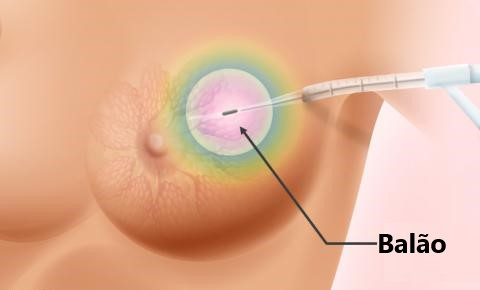
\includegraphics[width=0.8\textwidth]{Imagens/esquemaBalaoMama.jpg}
				\caption{Esquema de um tratamento de Braquiterapia de Mama utilizando um balão como aplicador.}
				\label{img:esquemaBalao}
			\end{figure}


			Em situações onde o PTV está próximo da pele ou da parede toráxica, é exigida uma assimetrida na distribuição de dose que só é alcançada comprometendo a dose no alvo (PTV), perdendo cobertura de dose no alvo ou aumentando as doses nos Orgãos de Risco (OARs).


			A prescrição de dose é feita a 1 cm do balão, portanto o raio do balão irá influenciar na dose na superfície do balão e consequentemente no gradiente de dose na região do alvo. Um balão com um diâmetro de 4.5 cm tem em sua superfície uma dose de aproximadamente 200\% da dose prescrita; quanto maior o diâmetro do balão, menor a dose na superfície do balão e vice-versa;

			A sutil anisotropia ao longo da direção do fio que conduz a fonte para as posições de para pode ser suavizada utilizando múltiplos tempos de parada (carregamento não uniforme). 

			Em teoria, quanto maior o diâmetro do balão, mais uniforme será a dose no PTV, pois a região de tratamento será deslocada para uma região de menor gradiente de dose. No entanto, alguns centros reportaram uma maior incidência na formação de seromas e cecroses gordurosas ao utilizar balões com maiores volumes preenchidos.

			O plano de tratamento é feito com o balão inflado e portanto é importante avaliar o estado do balão antes de cada fração para evitar superdosagem no alvo. Esta avaliação pode ser realizada através de imagens de ultrasonografia, fluoroscopia ou Tomografia Computadorizada.

			Os balões multi-lumen foram desenvolvidos para contornar o problema obtido com os balões com um único lumen central: Proteger os OARs sem comprometer a cobertura do PTV. Exemplos dos balões Multi-lumens são o ConturaMLB e o MammoSiteML. Ambos mativeram o lumen central mas adicionaram lumens extras deslocados a prtir do centro. 

			A maior vantagem em utilizar dispositivos multi-lumen está do desacoplamento da cobrtura do alvo com a proteção dos órgãos de risco que é inevitável utilizando apenas um lumen central. Com os balões Multi-lumen é possível criar distribuições de dose assimétricas que conformam melhor os PTV's assimétricos. Porém ao criar uma distribuição de dose assimétrica a partir de um balão simétrico, será criada regiões de dose dentro do volume alvo recebendo uma dose de radiação maior que a dose de prescrição.

			Os 3 balões\footnote{Ambos são comercializados pela empresa: Hologic Inc., Bedford, MA} mais utilizados são descritos abaixo:
			
			\begin{itemize}
				\item \textbf{\textcolor{CarnationPink}{MammoSite}}
				
					A    \ref{img:mammosite} mostra o balão e seus componentes. Este aplicador é constituído por um balão de silicone conectado por uma haste; possui um único lúmen por onde passa a fonte HDR e está disponível em dois tamanhos: 4.0 - 5.0 cm e 5.0 - 6.0 cm.

					\begin{figure}[h]
						\centering
						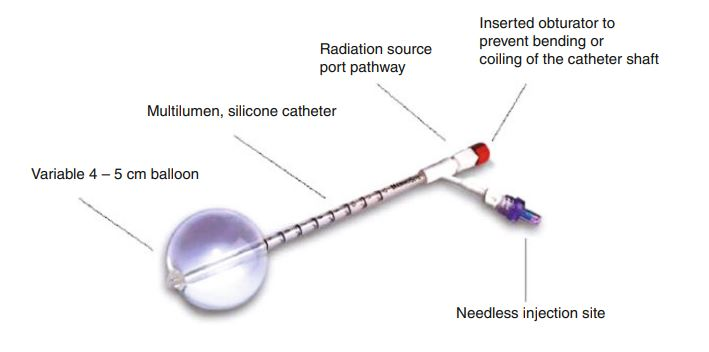
\includegraphics[width=0.6\textwidth]{Imagens/balaoMammoSite.JPG}
						\caption{MammoSite}
						\label{img:mammosite}
					\end{figure}

				\item \textbf{\textcolor{CarnationPink}{MammoSiteML}}
				
					A    \ref{img:mammositeml} mostra o balão e seus componentes. Este aplicador está disponível no tamanho de 3.5 - 5.0 cm e possui 4 lumens, sendo 1 lumen central e 3 lumens periférficos distibuídos em forma triangular à 0.3 cm do lúmen central.

					\begin{figure}[h]
						\centering
						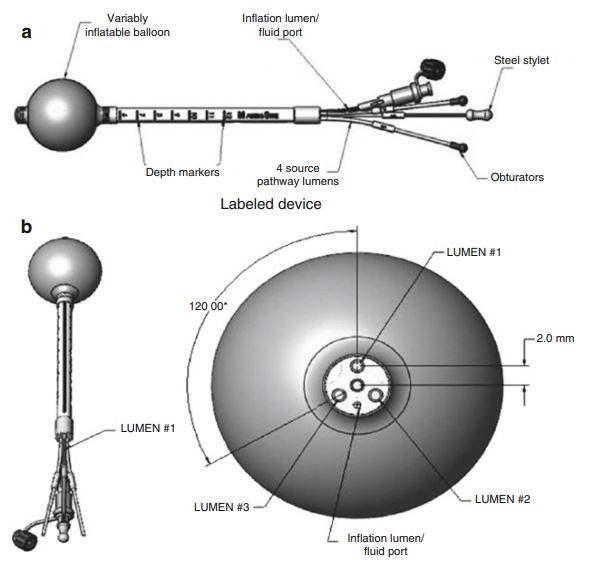
\includegraphics[width=0.65\textwidth]{Imagens/mammositeML.JPG}
						\caption{MammoSiteML}
						\label{img:mammositeml}
					\end{figure}

				
				\item \textbf{\textcolor{CarnationPink}{ConturaMLB}}
					
					A    \ref{img:conturaMLB} mostra os componentes deste aplicador. Está disponível nos tamanhos de 4 - 5 cm e 4.5 - 6 cm. Possui 5 lumens sendo 1 lumen central e outros 4 lumens periféricos igualmente espaçados a 0.5 cm de dustância do lúmem central. Possui duas portas de vácuo, nas partes proximal e distal do balão, que podem ser utilizadas para a remoção de ar ou fluido, aumentando a conformidade do tecido com a superfície do balão.
					
					\begin{figure}[h]
						\centering
						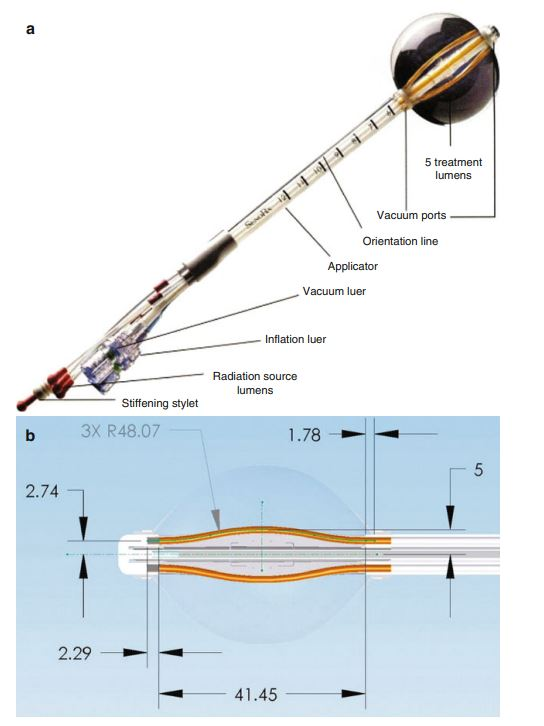
\includegraphics[width=0.45\textwidth]{Imagens/conturaMLB.JPG}
						\caption{ConturaMLB}
						\label{img:conturaMLB}
					\end{figure}
				\end{itemize}
			
			Os balões são inflados com uma solução salina e uma pequena quantidade de contraste para melhorar sua visualização. E para cada dispositivo é oferecido um balão para a avaliação do tamanho da cavidade, \textcolor{CarnationPink}{Cavity Evaluation Device (CED)} que deve ser colocado no momento da mastectomia e somente no momento de tratamento ele é substituído por um balão de tratamento.

			Outo aplicador disponível no mercado é chamado de \textcolor{CarnationPink}{Axxent}, que se trata de um balão desenvolvido com a braquiterapia eletrônica de 50 KeV (Xoft, Inc., Sunnyvale, CA) e semelhantemente ao MammoSite, possui apenas um único lumen central,    \ref{img:axxent}.

			\begin{figure}[h]
				\centering
				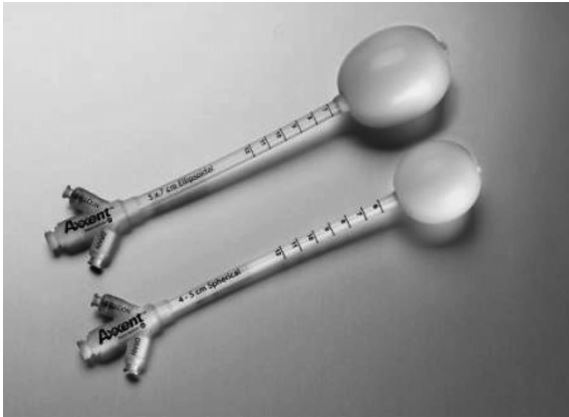
\includegraphics[width=0.45\textwidth]{Imagens/axxent.JPG}
				\caption{Aplicador Axxent}
				\label{img:axxent}
			\end{figure}

		








	\pagebreak
	\bibliography{ref.bib}

\end{document}